

\newpage
\tikz[remember picture,overlay]\node[opacity=1,inner sep=0pt] at (current page.center)%
{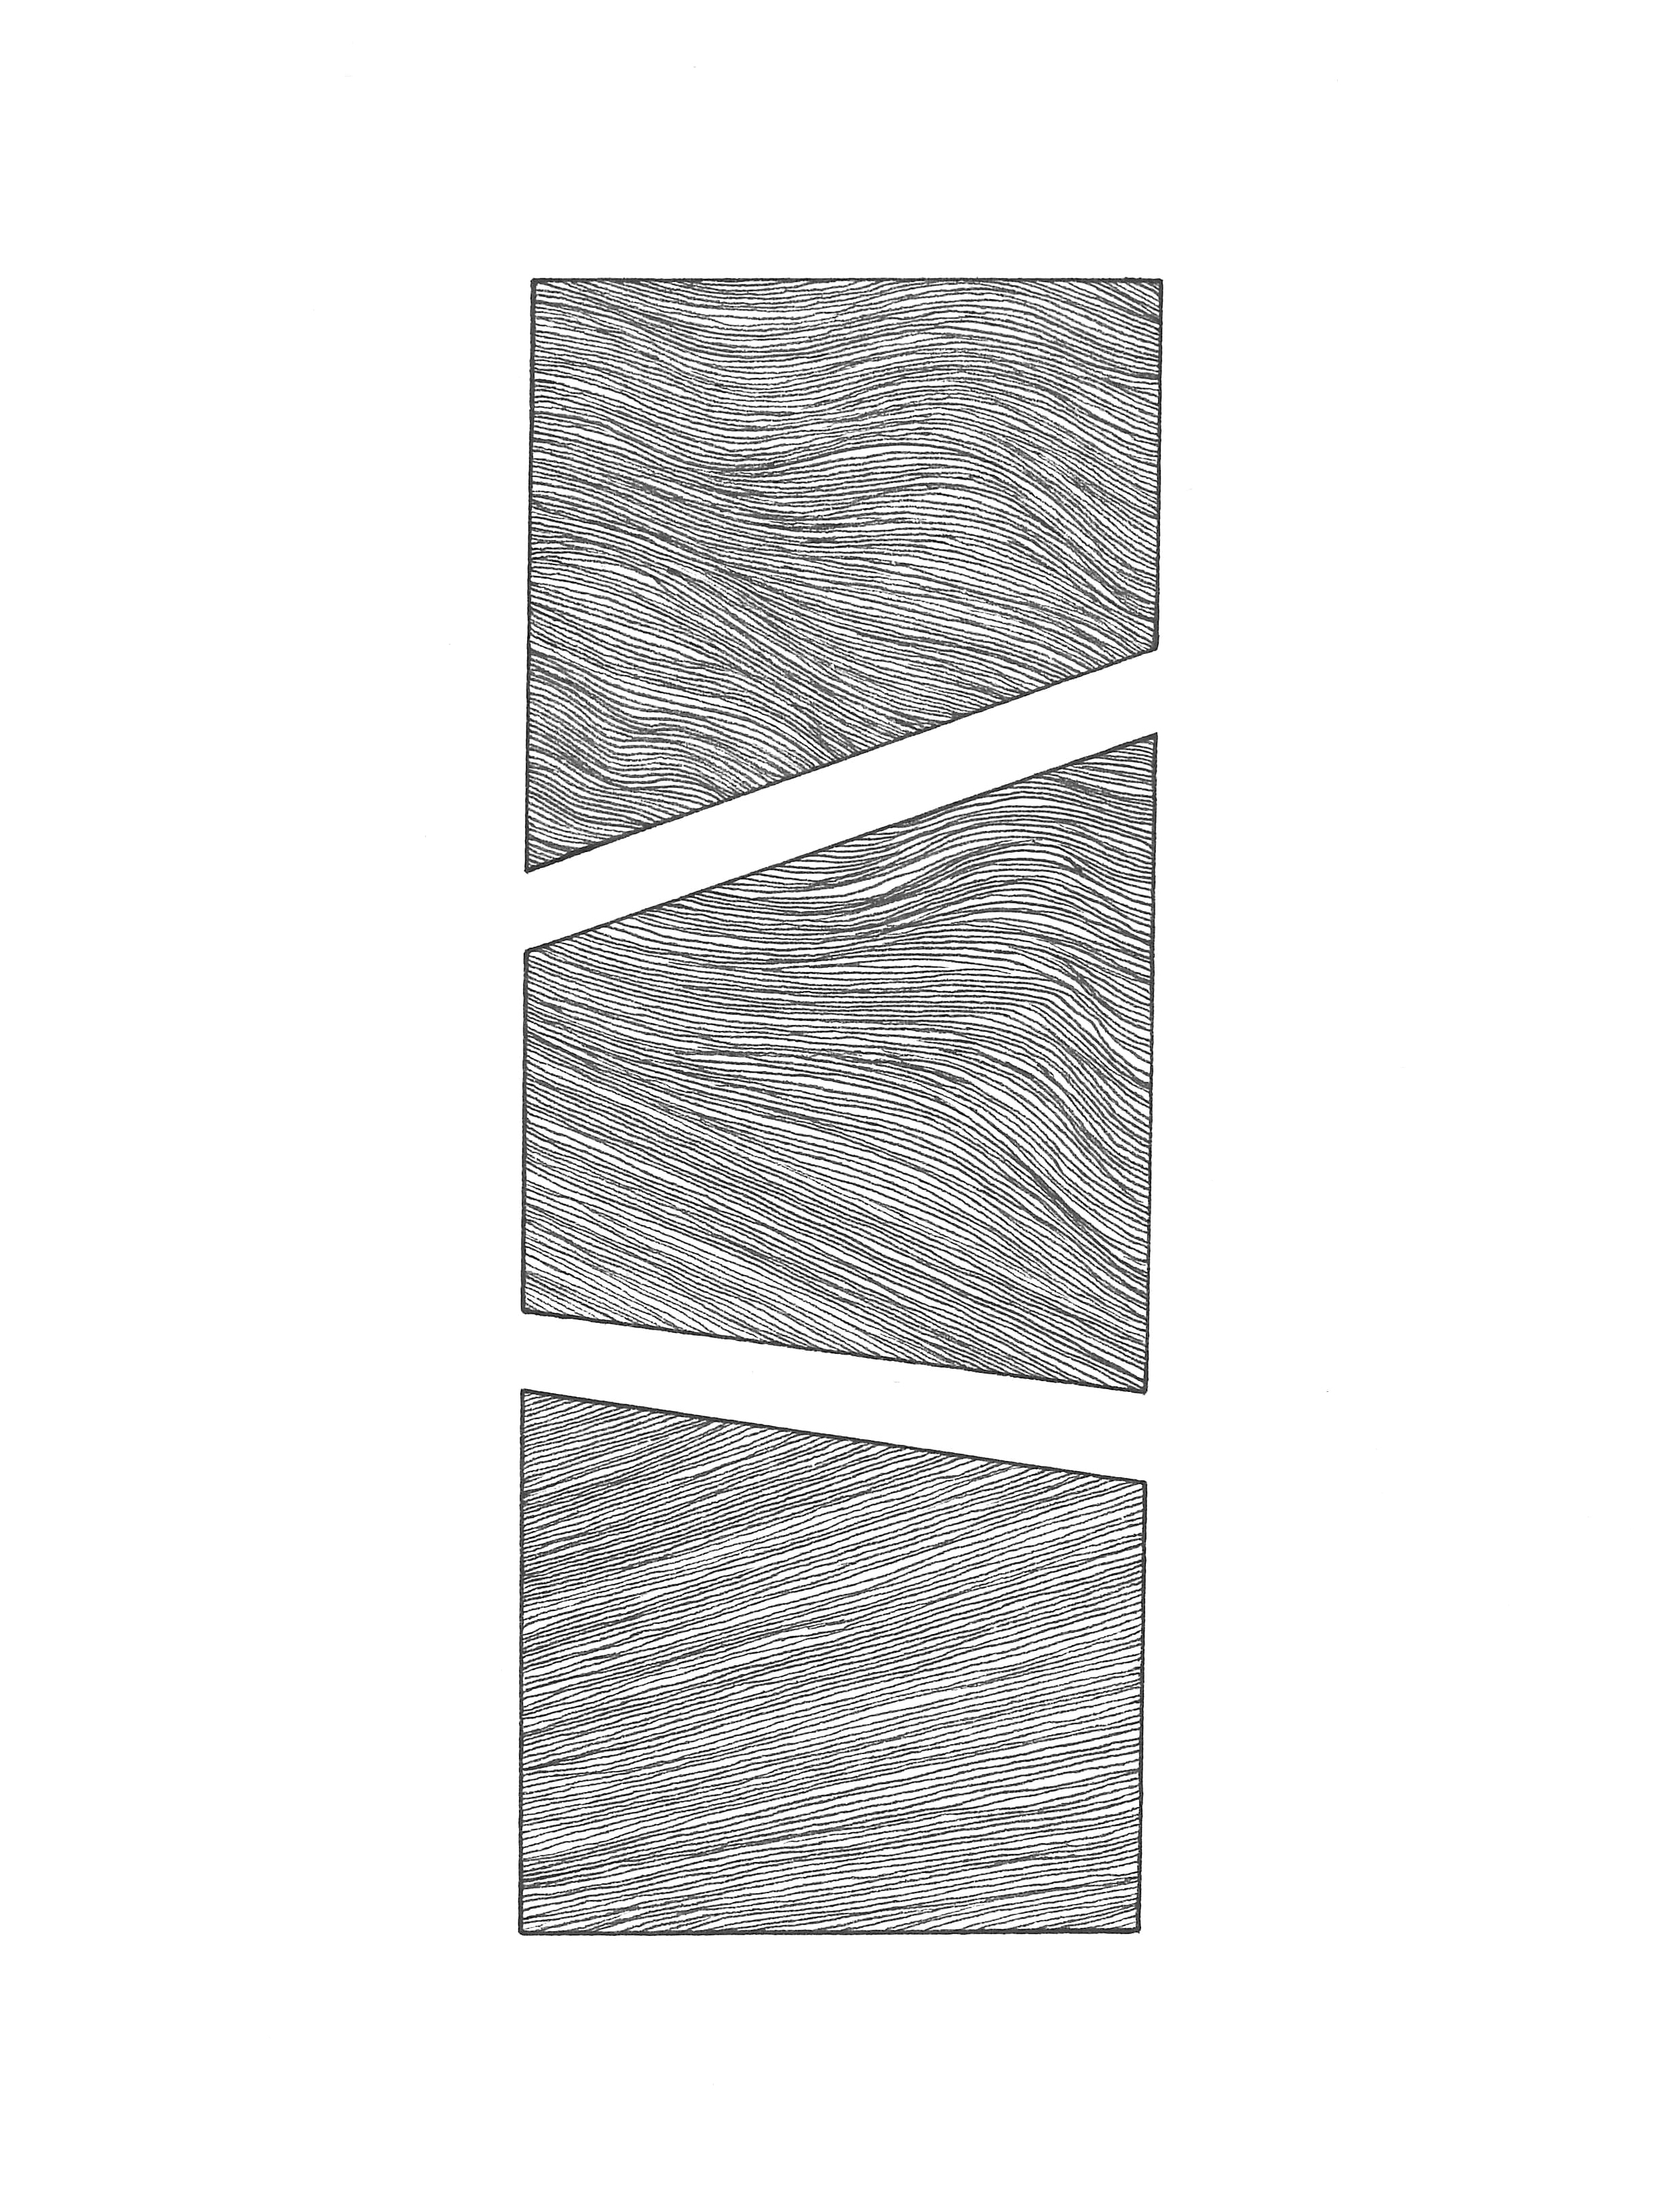
\includegraphics[%
clip,
width=1.05\paperwidth,
height=1.05\paperheight
]{chaptertitles/drawing3.jpeg}};

\clearpage


%\subsection*{Description}

\vspace*{2em}

{\par\centering {\Large \textbf{Description:}}\par}
\vspace{-2em}
\rule[-11pt]{\textwidth}{1pt}
\rule{\textwidth}{0.5pt}
    
The main result of the third paper concerns a connection between three different related mathematical worlds, called the stable, the prestable and the abelian world. These are all connected by something called a $t$-structure, and one can travel between them along this structure. The former world has no restrictions in its fluidity, while the second is restricted in one direction and the latter in both. We have tried to convey this distinction in the drawing by varying the use of curved and straight lines. 

\rule{\textwidth}{0.5pt}
\rule[11pt]{\textwidth}{1pt}



\newpage